\documentclass[aspectratio=169]{beamer}
\usetheme{Madrid}
\usepackage{booktabs}
\usepackage{graphicx}
\usepackage{array}

\title{Branch Specialization Checkpoint}
\subtitle{Two-Attractor Layout Test}
\author{Branch Specialization Project}
\date{2026-05-22}

\begin{document}

\begin{frame}
  \titlepage
  \vspace{-0.5em}
  \begin{center}
    Checkpoint reason: negative result separates specialization from modularity.
  \end{center}
\end{frame}

\begin{frame}{Question}
  \textbf{Current mechanism:} heterogeneous head dimensions create capacity-attractor slots.

  \vspace{0.8em}
  The next implication was:

  \begin{quote}
    If one high-capacity slot causes role competition, then two high-capacity
    slots should let local and induction split more cleanly.
  \end{quote}

  \vspace{0.8em}
  This checkpoint tests that implication under the strongest competition setting:
  local weight 0.25, induction weight 1.0.
\end{frame}

\begin{frame}{Setup}
  \begin{itemize}
    \item Same local-vs-induction toy task.
    \item Role score: single-head causal ablation loss delta.
    \item Two-48 layouts: [16,48,48,16], [48,16,48,16], [48,48,16,16].
    \item Control: \texttt{uniform2 = [64,64]}.
    \item Comparison baseline: prior single-64 heterogeneous layouts at local weight 0.25.
    \item Five seeds per new config.
  \end{itemize}
\end{frame}

\begin{frame}{Main Evidence}
  \begin{center}
  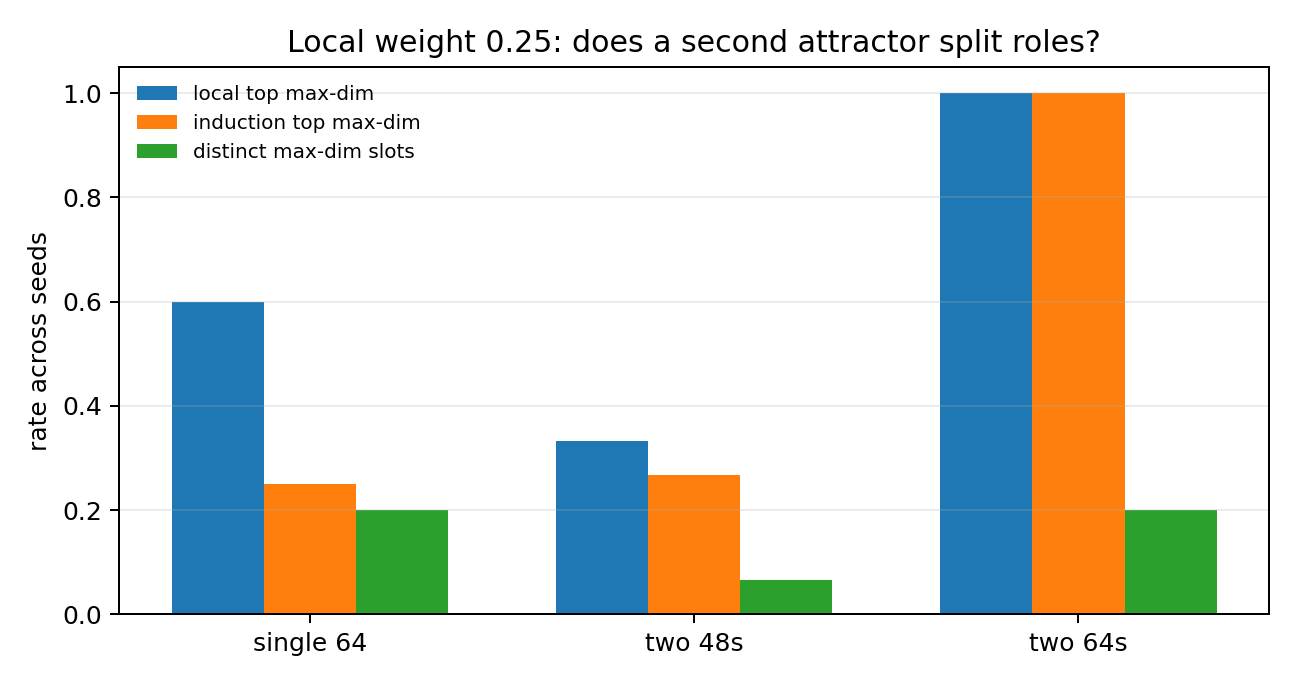
\includegraphics[width=0.86\linewidth]{figures/two_attractor_summary.png}
  \end{center}

  \vspace{-0.3em}
  \small
  The two-48 layouts did not make local and induction split between max-dim heads.
\end{frame}

\begin{frame}{Summary Table}
  \begin{center}
  \scriptsize
  \begin{tabular}{lrrrrr}
    \toprule
    Family & Models & Local top max & Induction top max & Same slot & Distinct max slots \\
    \midrule
    Single 64 hetero & 20 & 0.60 & 0.25 & 0.45 & 0.20 \\
    Two 48 hetero & 15 & 0.33 & 0.27 & 0.80 & 0.07 \\
    Two 64 uniform & 5 & 1.00 & 1.00 & 0.80 & 0.20 \\
    \bottomrule
  \end{tabular}
  \end{center}

  \vspace{0.7em}
  For two-48 layouts, local top heads were 48-dim in only 5/15 models and
  induction top heads were 48-dim in only 4/15 models.
\end{frame}

\begin{frame}{Interpretation}
  \textbf{Supported:}
  \begin{itemize}
    \item Adding more capacity does not automatically produce modular role separation.
    \item Local and induction can cohabit the same top causal slot.
    \item Differentiated capacity is insufficient evidence for functional modularity.
  \end{itemize}

  \vspace{0.6em}
  \textbf{Not supported:}
  \begin{itemize}
    \item Two medium-large heads are enough to make local and induction split roles.
    \item Two 64-dim heads necessarily split roles; \texttt{uniform2} shared the same top slot in 4/5 seeds.
  \end{itemize}
\end{frame}

\begin{frame}{Updated Claim}
  The Stage 3 claim should now be:

  \vspace{0.7em}
  \begin{quote}
    Structural heterogeneity can stabilize functional specialization slots, but
    functional modularity requires more than differentiated head capacity.
  \end{quote}

  \vspace{0.7em}
  This sharpens the central distinction:

  \begin{center}
    \textbf{specialization does not imply modularity}
  \end{center}
\end{frame}

\begin{frame}{Decision}
  Continue, but shift the next test from capacity heterogeneity to structural separation.

  \vspace{0.8em}
  Recommended next tests:
  \begin{itemize}
    \item Add explicit branch isolation or routing and compare against head-dimension heterogeneity.
    \item Use a more conflict-heavy two-role task where one shared head is less likely to solve both roles.
    \item Add multi-head ablation or path patching to distinguish role cohabitation from redundant separate circuits.
  \end{itemize}
\end{frame}

\begin{frame}{Sources and Provenance}
  \scriptsize
  \begin{itemize}
    \item Report: \texttt{doc/phase3\_toy\_competition\_two\_attractor.md}
    \item Training script: \texttt{scripts/toy\_competition\_head\_dim\_intervention.py}
    \item Analysis script: \texttt{scripts/analyze\_competition\_two\_attractor.py}
    \item New outputs: \texttt{results/phase3\_toy\_competition\_two48\_lw025/}
    \item Control output: \texttt{results/phase3\_toy\_competition\_uniform2\_lw025/}
    \item Combined analysis: \texttt{results/phase3\_toy\_competition\_two\_attractor/}
  \end{itemize}
\end{frame}

\end{document}
